\chapter{OpenGL}
OpenGL原生接口是C和C++的，不过OpenGL也提供了python版本

\section{安装}
为了用Python使用OpenGL，我们需要安装两个库：
\begin{enumerate}[label=\arabic*)]
    \item PyOpenGL：OpenGL的python接口库
    \item PyOpenGL\_accelerate：对PyOpenGL进行加速的库
\end{enumerate}

\begin{lstlisting}[style=demostyle,numbers=none]
conda create -n opengl_env python=3.10
conda activate opengl_env
# pip uninstall PyOpenGL PyOpenGL_accelerate
pip install PyOpenGL==3.1.7 PyOpenGL_accelerate==3.1.7
pip install glfw
\end{lstlisting}

\begin{lstlisting}[style=pythonstyle, title={绘制三角形.py}]
import glfw
from OpenGL.GL import *
import sys

def main():
    if not glfw.init():
        sys.exit(1)

    window = glfw.create_window(400, 400, "Hello Triangle", None, None)
    if not window:
        glfw.terminate()
        sys.exit(1)

    glfw.make_context_current(window)
    glClearColor(0.2, 0.3, 0.3, 1.0)  # 设置清除色为深绿色

    while not glfw.window_should_close(window):
        glClear(GL_COLOR_BUFFER_BIT)

        # --- 开始绘制 ---
        glBegin(GL_TRIANGLES)
        glColor3f(1.0, 0.0, 0.0)   # 红色
        glVertex2f(0.0, 0.5)       # 上顶点
        glColor3f(0.0, 1.0, 0.0)   # 绿色
        glVertex2f(-0.5, -0.5)     # 左下
        glColor3f(0.0, 0.0, 1.0)   # 蓝色
        glVertex2f(0.5, -0.5)      # 右下
        glEnd()
        # --- 绘制结束 ---

        glfw.swap_buffers(window)
        glfw.poll_events()

    glfw.terminate()

if __name__ == "__main__":
    main()
\end{lstlisting}
\begin{figure}[htpb]
    \centering
    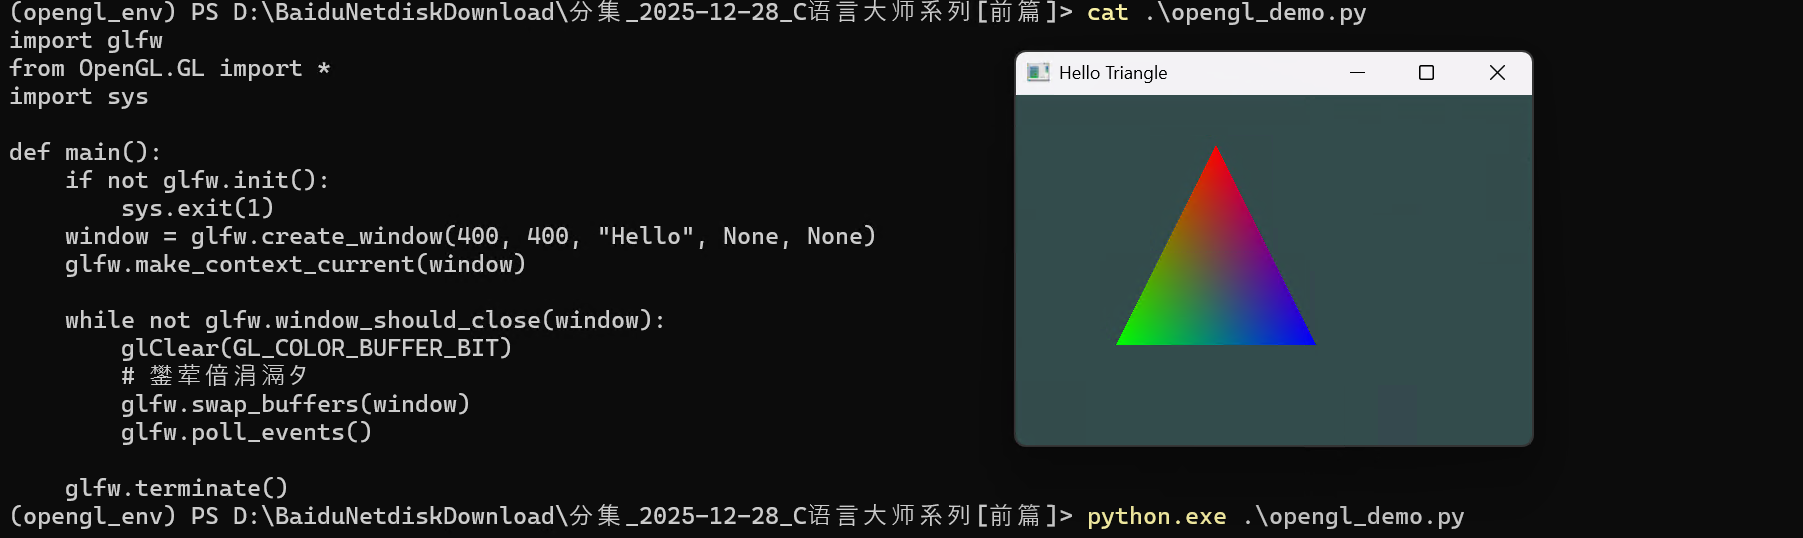
\includegraphics[width=0.6\textwidth]{part/图形化/opengl/pic/概述/安装成功简单demo.png}
    \caption{安装成功的简单Demo}
    \label{fig:install_success_demo}
\end{figure}

